%%%%%%%%%%%%%%%%%%%%%%%%%%%%%%%%%%%%

\section{4.1. Estimativas pontuais e variabilidade de amostragem}

%%%%%%%%%%%%%%%%%%%%%%%%%%%%%%%%%%%%

\begin{frame}
\frametitle{Estimativas pontuais e erro}
\justifying

\begin{itemize}
    \justifying
    \footnotesize
    \item Frequentemente estamos interessados em \hl{parâmetros populacionais}.
    \item É difícil coletar todos os dados de uma população (fazer um censo). Por isso usamos \hl{estatísticas da amostra} como \hl{estimativas pontuais} dos parâmetros desconhecidos da população de interesse.
    \item \hl{Erro} na estimativa = diferença entre o parâmetro da população e a estatística da amostra.
    \item \hl{Viés} é uma tendência sistemática que super ou subestima o verdadeiro parâmetro da população.
    \item \hl{Erro de amostragem} descreve o quanto uma estimativa tende a variar de uma amostra para outra.
    \item Grande parte das estatísticas concentra-se em compreender e quantificar o erro de amostragem, e o \hl{tamanho da amostra} é útil para quantificar esse erro.
\end{itemize}

\end{frame}

\begin{frame}
\justifying
\dq{Suponha que nós amostramos aleatoriamente 1.000 adultos de cada estado nos EUA. Você esperaria que as médias amostrais de suas alturas sejam as mesmas, um pouco diferentes ou muito diferentes?}

\pause
\justifying
\soln{Esperamos que as médias amostrais não sejam as mesmas, mas apenas um pouco diferentes.}

\end{frame}


\begin{frame}
\frametitle{}

\begin{center}
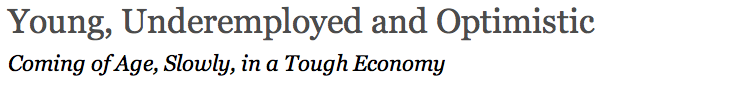
\includegraphics[width=0.95\textwidth]{4-1_var_in_est/pew1.png} \\
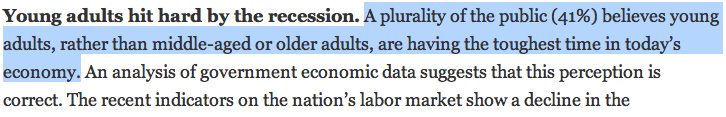
\includegraphics[width=0.95\textwidth]{4-1_var_in_est/pew2.png} \\
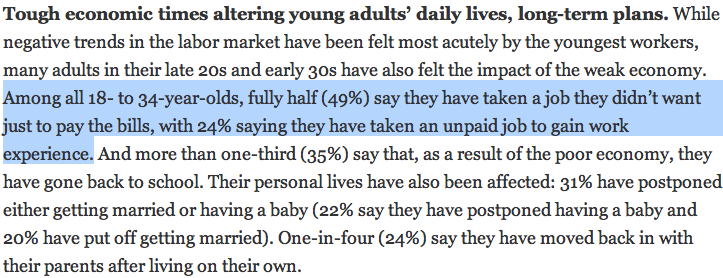
\includegraphics[width=0.95\textwidth]{4-1_var_in_est/pew3.png}
\end{center}

\ct{\webURL{http://pewresearch.org/pubs/2191/young-adults-workers-labor-market-pay-careers-advancement-recession}}

\end{frame}


%%%%%%%%%%%%%%%%%%%%%%%%%%%%%%%%%%%%

\begin{frame}
\frametitle{Tradução do texto: Young, Underemployed and Optmistic}
\justifying
\textbf{Jovem, Subempregado e Otimista}\\
\vspace{0.1 cm}

\justifying
\textit{Envelhecer, lentamente, em uma economia difícil}.\\
\vspace{0.4 cm}

\justifying
\footnotesize{
\textbf{Jovens adultos são duramente atingidos pela recessão}. \hl{Uma grande parte do público (41\%) acredita que os jovens adultos, ao invés dos adultos de meia-idade ou mais os velhos, estão tendo o momento mais difícil na economia atual}. Uma análise dos dados econômicos do governo sugere que essa percepção está correta. Os indicadores recentes sobre o mercado de trabalho da nação mostram um declínio na taxa de desemprego. No entanto, desde 2010, a proporção de jovens adultos de 18 a 24 anos atualmente empregados (54\%) é a menor desde que o governo começou a coletar esses dados em 1948. E a diferença no emprego entre os jovens e todos os adultos em idade ativa - 15 pontos percentuais - é o mais amplo da registrado na história. Além disso, os jovens adultos empregados em período integral tiveram uma queda maior nos seus ganhos semanais (menos 6\%) do que qualquer outro grupo etário nos últimos quatro anos.}\\

\end{frame}
%%%%%%%%%%%%%%%%%%%%%%%%%%%%%%%%%%%%

\begin{frame}
\frametitle{Tradução do texto: Young, Underemployed and Optmistic}

\justifying
\footnotesize{
\textbf{Tempos econômicos difíceis que alteram a vida cotidiana dos jovens adultos e seus planos de longo prazo}. Embora as tendências negativas no mercado de trabalho tenham sido mais fortemente sentidas pelos trabalhadores mais jovens, muitos adultos com cerca de 20 e 30 anos também sentiram o impacto da fraca economia. \hl{Entre todas as pessoas de 18 a 34 anos, metade (49\%) diz que aceitou um trabalho que não queria apenas para poder pagar as contas, com 24\% dizendo que aceitou um emprego não remunerado para ganhar experiência profissional}. E mais de um terço (35\%) dizem que, como resultado da economia pobre, voltaram à escola. Suas vidas pessoais também foram afetadas: 31\% adiaram o casamento ou a gravidez (22\% disseram que adiaram ter um bebê e 20\% adiaram o casamento). Um em quatro (24\%) dizem que voltaram a morar com os pais depois de viverem sozinhos.}

\end{frame}
%%%%%%%%%%%%%%%%%%%%%%%%%%%%%%%%%%%%

\begin{frame}
\frametitle{Margem de erro}

\begin{center}
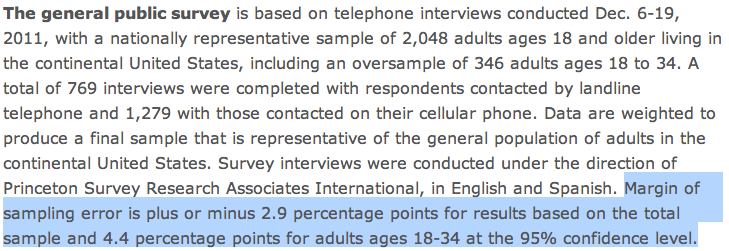
\includegraphics[width=0.95\textwidth]{4-1_var_in_est/pew4.png}
\end{center}

\end{frame}
%%%%%%%%%%%%%%%%%%%%%%%%%%%%%%%%%%%%

\begin{frame}
\frametitle{Tradução do texto: Margem de Erro}
\justifying
\small{
\textbf{A pesquisa do público geral} é baseada em entrevistas telefônicas realizadas de 6 a 19 de dezembro de 2011, com uma amostra nacionalmente representativa de 2.048 adultos com 18 anos ou mais vivendo nos Estados Unidos continental, incluindo uma sobreamostra de 346 adultos entre 18 e 34 anos. Um total de 769 entrevistas foram realizadas para os telefones fixos e 1.279 para os telefones celulares das pessoas. Os dados são ponderados para produzir uma amostra final que seja representativa da população geral de adultos nos Estados Unidos continental. As entrevistas da pesquisa foram conduzidas sob a direção da Princeton Survey Research Associates International, em inglês e espanhol. \hl{A margem de erro de amostragem é de mais ou menos 2,9 pontos percentuais para os resultados com base na amostra total e 4,4 pontos percentuais para os adultos com idades entre 18 e 34 anos, com nível de confiança de 95\%.}
}

\end{frame}
%%%%%%%%%%%%%%%%%%%%%%%%%%%%%%%%%%%%

\begin{frame}
\frametitle{Margem de erro}

\begin{itemize}
\justifying
\item 41\% $\pm$ 2.9\%: Estamos 95\% confiantes de que entre 38.1\% e 43.9\% do público acreditam que os jovens adultos, em vez de adultos de meia-idade ou mais velhos, estão tendo o momento mais difícil na economia atual.

\justifying
\item 49\% $\pm$ 4.4\%: Estamos 95\% confiantes de que entre 44.6\% e 53.4\% dos jovens entre 18 e 34 anos aceitaram um emprego que não queriam apenas para poder pagar as contas.

\end{itemize}

\end{frame}

%%%%%%%%%%%%%%%%%%%%%%%%%%%%%%%%%%%

\subsection{Exercício de aplicação}

%%%%%%%%%%%%%%%%%%%%%%%%%%%%%%%%%%%

\begin{frame}
\frametitle{Exercício de aplicação}
\justifying
\dq{O histograma a seguir mostra a distribuição do quantidade de bebidas que um grupo de estudantes universitários precisa ingerir para ficarem bêbados. Vamos supor que esta é a nossa população de interesse. Se selecionarmos aleatoriamente observações desse conjunto de dados, quais valores têm maior probabilidade de serem selecionados? E quais são os menos prováveis?}

\begin{center}
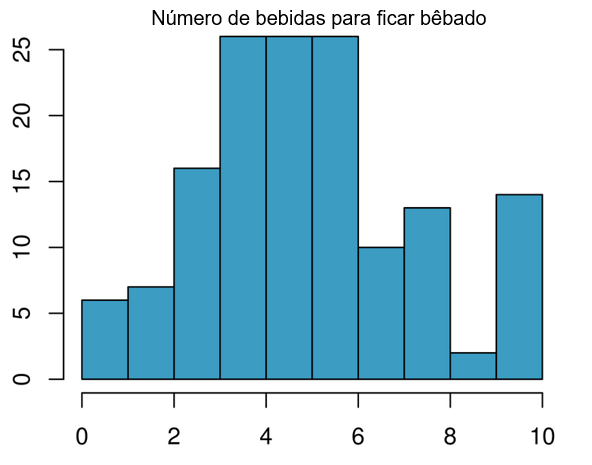
\includegraphics[width=0.4\textwidth]{4-1_var_in_est/no_drinks_drunk.png} 
\end{center}

\end{frame}

%%%%%%%%%%%%%%%%%%%%%%%%%%%%%%%%%%



\begin{frame}[fragile]
\frametitle{Exercício de aplicação}

\begin{center}
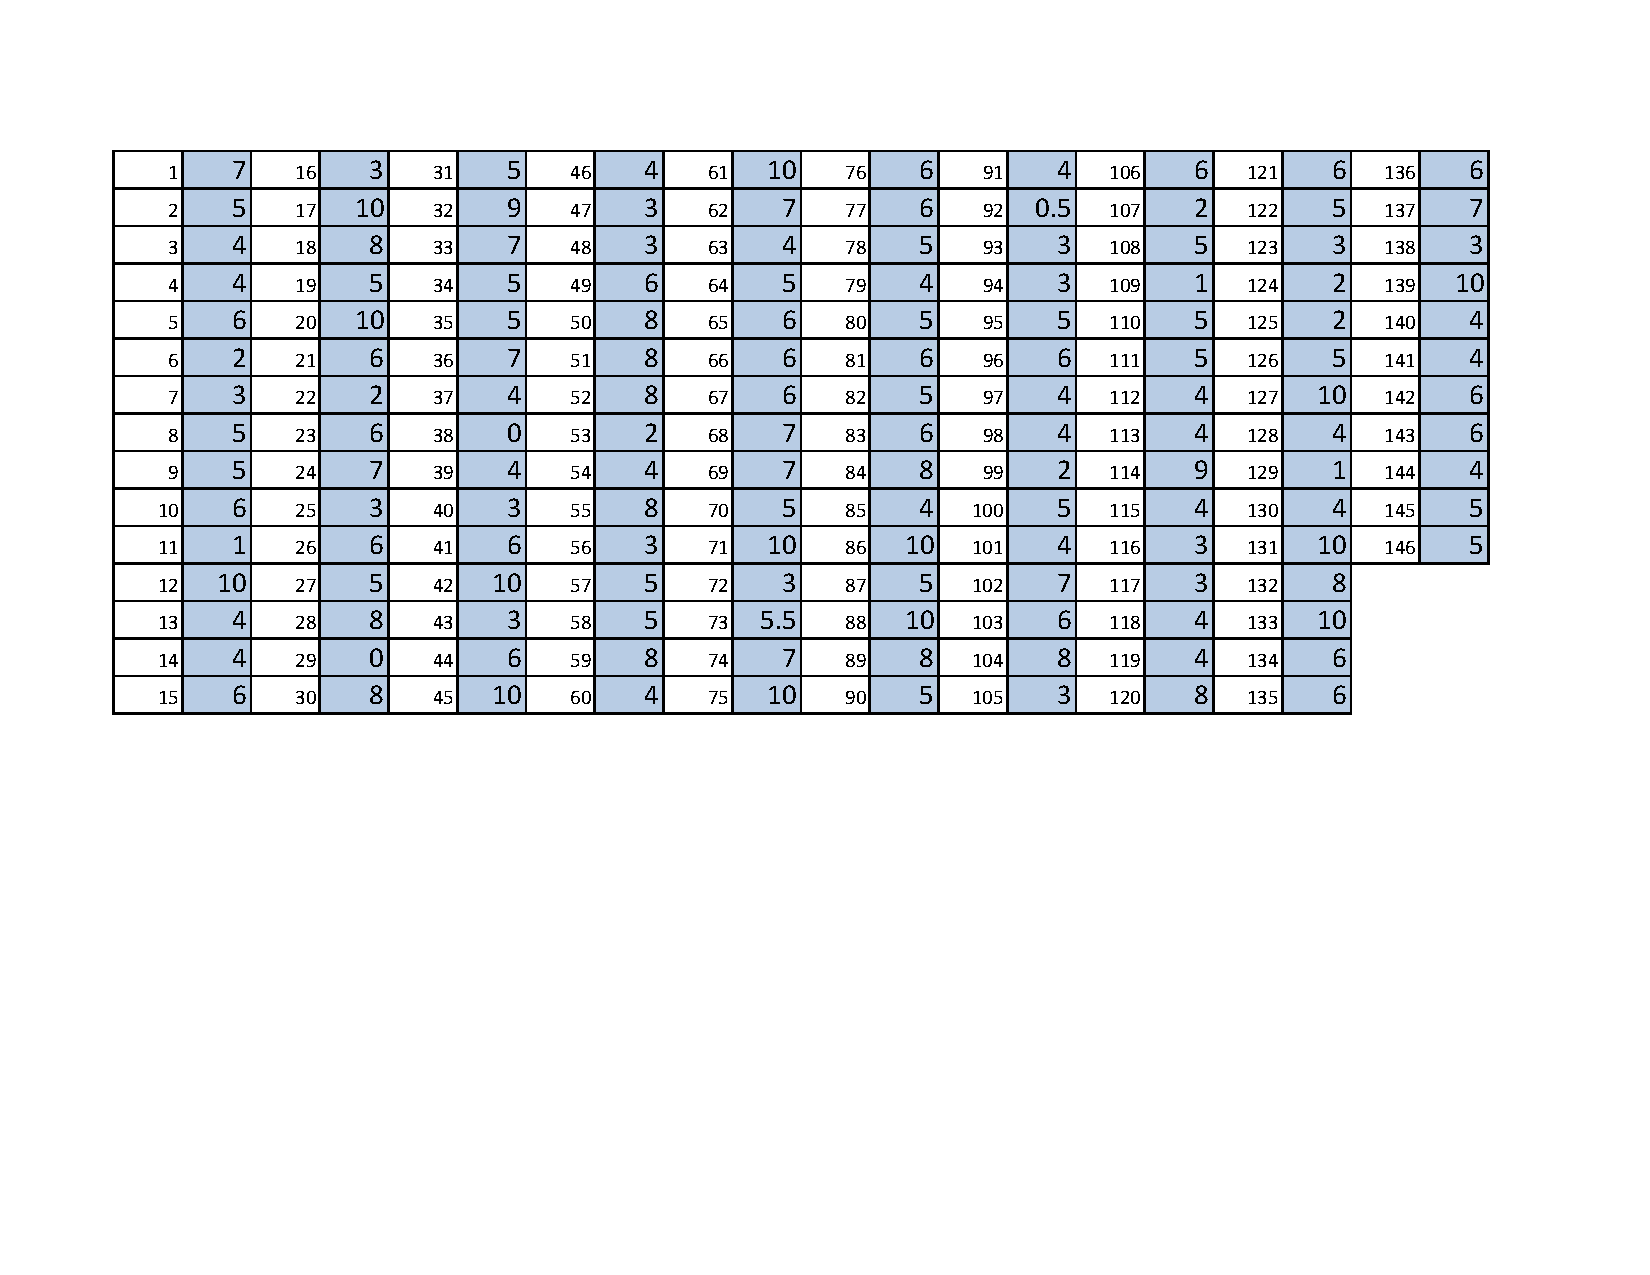
\includegraphics[width=1.05\textwidth]{4-1_var_in_est/no_drinks_drunk_clean.pdf} 
\end{center}

\end{frame}

%%%%%%%%%%%%%%%%%%%%%%%%%%%%%%%%%%%

\begin{frame}[fragile]
\frametitle{Exercício de aplicação}
\justifying
\dq{Exemplo:} Lista de números aleatórios: 59, 121,  88,  46,  58,  72,  82,  81,   5,  10 \\

\begin{center}
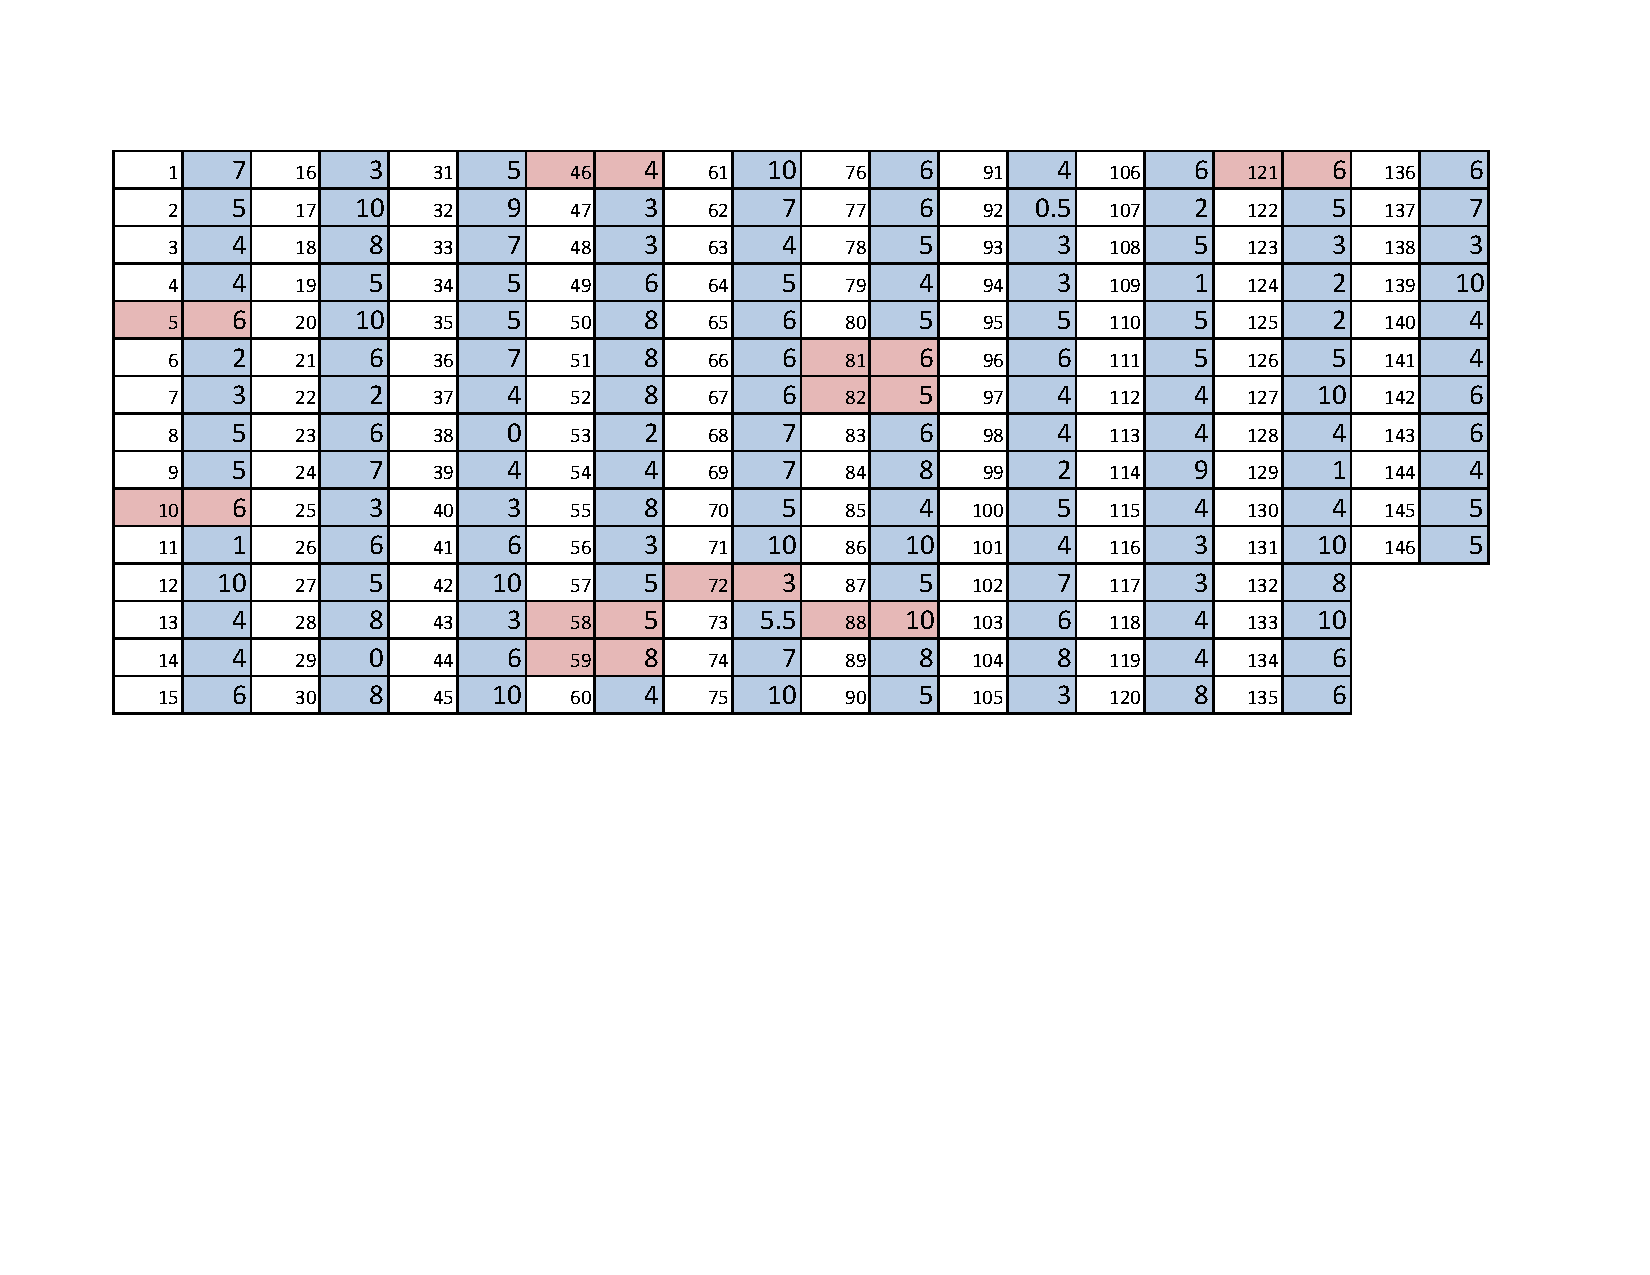
\includegraphics[width=0.9\textwidth]{4-1_var_in_est/no_drinks_drunk_marked.pdf} 
\end{center}

\pause
\justifying
Média da amostra: (8+6+10+4+5+3+5+6+6+6) / 10 = 5.9

\end{frame}

%%%%%%%%%%%%%%%%%%%%%%%%%%%%%%%%%


\begin{frame}[fragile]
\frametitle{Distribuição de amostragem}
\justifying
O que você acabou de construir é chamado de \hl{distribuição de amostragem}.

\pause

$\:$ \\
\justifying
\dq
{Qual é a forma e o centro dessa distribuição? Com base nessa distribuição, qual você acha que é a média real da população?}

$\:$ \\
\justifying
\soln{\only<3>{
Aproximadamente 5,39, a verdadeira média da população.
}}

\end{frame}


%%%%%%%%%%%%%%%%%%%%%%%%%%%%%%%%%%

\subsection{Distribuições de amostragem - via CLT}

%%%%%%%%%%%%%%%%%%%%%%%%%%%%%%%%%%

\begin{frame}
\frametitle{Teorema do limite central (TLC)}
\justifying
\formula{Teorema do limite central}
{A distribuição da média da amostra é bem aproximada por um modelo normal:
\[ \bar{x} \sim N \pr{ \text{média} = \mu, SE = \frac{\sigma}{\sqrt{n}} }, \]
onde SE representa \hl{erro padrão}, que é definido como o desvio padrão da distribuição amostral. Se $\sigma$ é desconhecido, use $s$.
}

\begin{itemize}
\justifying
\item Não foi uma coincidência que a distribuição de amostragem que vimos anteriormente fosse simétrica e centralizada na média real da população.
\end{itemize}
\end{frame}

%%%%%%%%%%%%%%%%%%%%%%%%%%%%%%%%%%

\begin{frame}
\frametitle{Teorema do limite central (TLC)}
\begin{itemize}
\justifying
\item Nós não vamos passar por uma prova detalhada do porquê $SE =  \frac{\sigma}{\sqrt{n}}$, mas note que conforme $n$ aumenta, $SE$ diminui. 
\begin{itemize}
\justifying
\item À medida que o tamanho da amostra aumenta, esperaríamos que as amostras produzissem médias de amostras mais consistentes, portanto a variabilidade entre as médias da amostra seria menor.
\end{itemize}

\end{itemize}

\end{frame}

%%%%%%%%%%%%%%%%%%%%%%%%%%%%%%%%%%%%

\begin{frame}
\frametitle{TLC - condições}
\justifying
Certas condições devem ser atendidas para o TCL valer:

\begin{enumerate}
\justifying
\footnotesize
\item \hlGr{Independência:} As observações da amostra devem ser independentes. \\
\justifying
Isso é difícil de verificar, mas é mais provável termos independência 
\begin{itemize}
\footnotesize
\justifying
\item quando amostragem/atribuição aleatória é realizada, e 
\justifying
\item quando é feita amostragem sem reposição, $n$ $<$ 10\% da população.
\end{itemize}

\pause
\justifying
\item \hlGr{Tamanho da amostra/assimetria:} A distribuição da população é normal ou, se a distribuição da população for assimétrica, o tamanho da amostra precisa ser grande.\\

\begin{itemize}
\footnotesize
\justifying
\item Quanto mais assimétrica a distribuição da população, maior o tamanho da amostra que precisamos para a aplicar TCL.
\justifying
\item para distribuições moderadamente assimétrica $n > 30$ é uma regra prática amplamente usada \\
\end{itemize}

Isso também é difícil de verificar para a população, mas podemos verificá-la usando os dados da amostra e assumir que a amostra espelha a população.

\end{enumerate}
\end{frame}

